\section{Candidate localization without a precise mass}
\label{sec:candidate-inventory}

Candidate selection and localization are useful results before an individual
mass is identified. They require distinct evidence labels: a \emph{supported
lensing event} has evidence for lensing; a \emph{black-hole search target}
justifies further investigation; a \emph{black-hole candidate} requires
specific evidence favoring that interpretation, with alternatives retained;
and a \emph{strongly supported identification} requires discriminating
evidence against relevant stellar and other compact-object explanations.
A precise mass is not required for a search target. Lensing itself is not
a black-hole classification, and nonrejection of one light-curve model is
not a comparison against source variability or other alternatives.
\emph{Review required} therefore remains an available outcome.

\subsection{A complete, versioned historical inventory}

The metadata inventory joins the complete 100-event pilot to all 59
published parallax events of Wyrzykowski et al.\ \cite{Wyrzykowski2015,Wyrzykowski2016}.
Four shared identities---0264/PAR-07, 0568/PAR-21, 2122/PAR-37 and
3404/PAR-17---are independently checked using database identifiers,
published aliases and compatible catalog directions. The union contains
155 events. It retains all 89 inadequate pilot fits, all 11 scalar-screen
nonrejections and both stricter frozen follow-up qualifications.
The parallax cohort retains all 142 published degenerate model summaries;
they are literature metadata, not additional observations.
Its 13 historical dark-remnant-consistent events are not 13 black holes:
that category includes white dwarfs and neutron stars and depends on the
adopted Galactic and relative-motion assumptions \cite{Wyrzykowski2016}.

Twenty-six exact database matches have independently hash-verified older
2015 photometry: 23 optimized Class A tables and three Class B tables,
containing 19\,068 rows. The remaining 33 entries stay explicitly
unavailable. These older tables are not asserted equivalent to the
2016 reduction, calibration or outlier masks. No new parallax fit,
population inference or follow-up ranking is performed by this inventory.
The earlier pilot ranking remains separately versioned.

\begin{table}[tbp]
\centering\small
\caption{Three investigation targets with distinct evidential bases.
Coordinates are printed catalog source/event directions, with J2000
equinox; an observing epoch or current lens position is not supplied.
No row is an accepted new black-hole identification.}
\label{tab:atlas-targets}
\begin{tabular}{@{}lllp{.40\linewidth}@{}}
\toprule
OGLE3-ULENS & RA (h:m:s) & Dec (d:m:s) & Basis and limitation\\
\midrule
0585 & 17:48:45.32 & $-$34:44:43.8 &
Frozen photometric follow-up screens; mass and lens type unresolved.\\
3092 & 18:04:17.03 & $-$27:36:35.8 &
Same screens; known OGLE-2007-BLG-057/MOA-2007-BLG-027 event.\\
PAR-13 & 17:35:55.95 & $-$27:16:02.1 &
Disputed prior-conditional BH-scale interpretation; unreliable source
astrometry and a lower-mass alternative.\\
\bottomrule
\end{tabular}
\end{table}

\subsection{Literature revisions and localization limits}

The two pilot targets in Table~\ref{tab:atlas-targets} are qualified
archival follow-ups, not evidence that black holes are preferred.
PAR-13 enters as a disputed literature search target. The later analysis
of Mr\'oz and Wyrzykowski \cite{Mroz2021} revises several earlier
mass interpretations: PAR-02, historically the strongest black-hole
candidate, is favored to be a roughly $0.9\,M_\odot$ bulge star under
their fiducial priors. Their BH-scale PAR-13 inference depends on a
Gaia DR2 source solution with RUWE 1.67, absent from EDR3; an alternative
OGLE source proper motion gives a lower conditional mass. These
conflicting, prior-dependent interpretations remain attributed literature
records. They are neither independent lens-mass measurements nor optimizer
targets. None of the 155 entries is promoted to the candidate or strongly
identified black-hole tier by the tracker.

\begin{figure}[tbp]
\centering
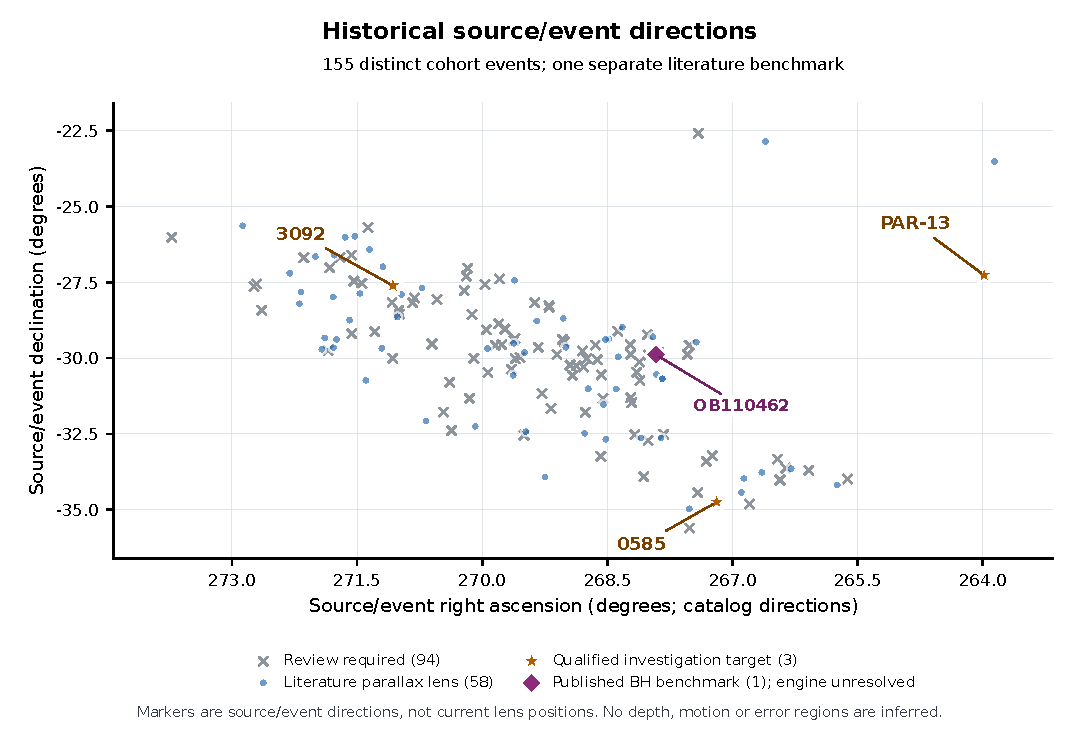
\includegraphics[width=.97\linewidth]{../figures/candidate_inventory_sky.pdf}
\caption{Historical source/event directions in the 155-event union,
with the separate published OB110462 benchmark optionally included
(156 markers in total). Supported-lens labels are inherited from the
published parallax study; review labels preserve the pilot's unresolved
assessments. The three search targets have different qualifications
(Table~\ref{tab:atlas-targets}). Markers are not present-day lens positions;
angular uncertainty regions, depth and propagation are unavailable.
Survey selection and alignment affect this footprint: an unmarked region
does not imply absence of black holes.}
\label{fig:candidate-inventory-sky}
\end{figure}

Source/event direction, inferred lens position at a stated epoch, and
three-dimensional position are separate outputs. A J2000 catalog label
specifies an equinox, not an observation epoch or proper-motion
correction. Every newly inferred lens position, uncertainty, mass,
distance, absolute proper motion and radial velocity remains null here;
no three-dimensional or propagated lens marker is supplied.
OGLE-2011-BLG-0462/MOA-2011-BLG-191 is a separate published positive
benchmark \cite{Sahu2025}. Its strong identification is labeled
\emph{literature}; the tracker's joint recovery remains unestablished.
The published full analysis is not certified by importing that label.
BHSM interpretation remains one ordinary compact-lens Einstein/GHY
exterior response counted once; these directions and screening results
identify no core state, membrane deformation or horizon.

\subsection{Usable and auditable metadata replay}

The app, \texttt{blackhole-tracker atlas} commands and Python interface
expose the same retained inventory, aliases, quality flags and evidence
layers. Filters select a view without deleting unselected or failed
records. A portable standard-library builder reruns association and
classification rules from factual metadata snapshots, with no original
observation redistribution or new likelihood call. Two assemblies are
byte-identical; relocation tests forbid reads of the original source
paths. Browser--Python replay preserves the exact UTF-8 inventory text,
including line endings, and checks selected records against the complete
inventory. SHA-256 establishes byte consistency, not authenticity,
scientific adequacy or black-hole certification. The software,
metadata and reviewer materials cite the
\href{https://github.com/ncarberry64/Berger-Hopf-Standard-Model}{formal BHSM repository}.
